
\chapter{Software Architecture and Simulation Environments}

This chapter discusses the software architecture of the mobile manipulation robotic system and the simulation 
environments used for testing and development. The software architecture is based on the Robot Operating System 2 (ROS2)
middleware, which provides a flexible and modular framework for developing robotic applications. 
The simulation environments are based on Rviz2 and Ignition Gazebo, which provide realistic simulation environments
for testing the algorithms before deployment on the real robots.

\section{ROS2 Control Interface for Igus Rebel Arm}

The first step in developing the software architecture for the mobile manipulation robotic system is to interface the
Igus Rebel Arm with ROS2. The Igus Rebel Arm is a 6-DOF robotic arm that can be controlled by either the CAN binary bus
or the Ethernet interface (proprietary CRI protocol). The CAN bus interface is used for low-level access to the arm's
joints, while the Ethernet interface is used for high-level control and monitoring of the arm's state. 
The ROS2 control interface for the CAN bus was already implemented by the manufacturer \textit{Commonplace Robotics},
but the requirement was the development of a ROS2 control interface for the Ethernet interface since the CAN bus interface
requires a proprietary cable, which is not available to me. Using the Ethernet interface makes it easier to 
plug it into the switch and control the arm from any computer on the local network.

Developing the \textbf{ROS2 control interface} for the Ethernet interface required understanding the CRI protocol, which
is a protocol based on string messages. The CRI protocol is used to send commands to the arm in the form of
joint positions or velocities (jogs) and to receive feedback from the arm in the form of joint positions.
Controlling the cobot using ROS2 requires a hardware interface, used to command and control the robot by interfacing
with the hardware via the \textbf{CRI protocol}. The hardware interface is implemented as a ROS2 lifecycle node that
is interfaced directly with the Joint Trajectory Controller, which is a ROS2 controller that can be used to
control the arm using joint trajectory messages. This controller is then handled by MoveIt2, which is a ROS2
motion planning framework that can be used to plan and execute trajectories for the arm.

%Add a figure of the control architecture
\begin{figure}[t]
    \centering
    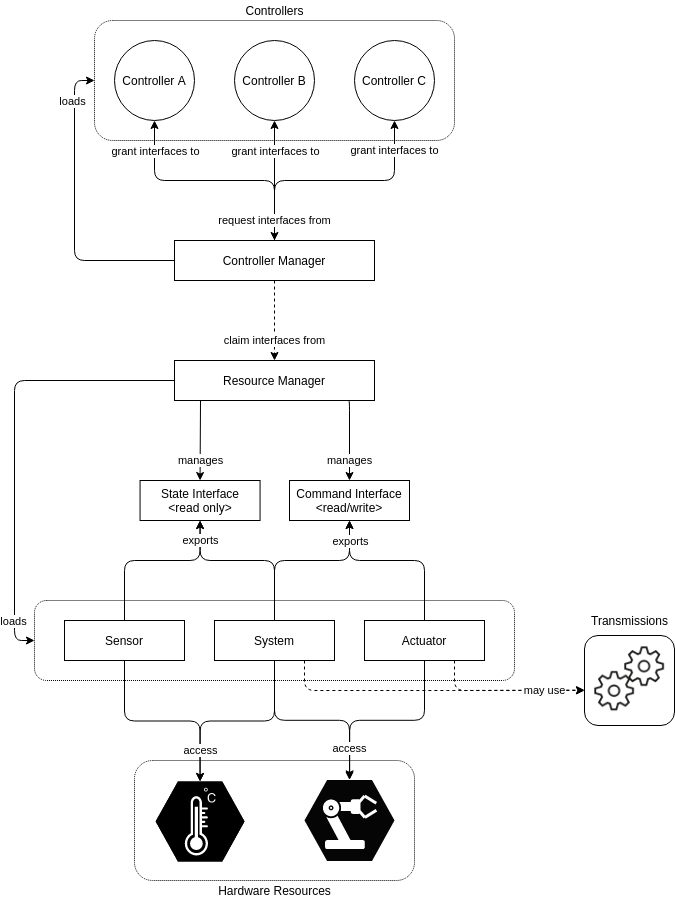
\includegraphics[width=0.6\textwidth]{c4_04.png}
    \caption{ROS2-Control Architecture example}
    \label{fig:ros2control}
\end{figure}

The diagram in figure \ref{fig:ros2control} shows an overview of how \textit{ROS2-Control} works.
The hardware interface implemented for controlling the Igus ReBel arm is a ROS2 lifecycle \textit{System Interface},
which is a type of interface that supports joints and actuators. The system interface accesses the hardware
via the CRI protocol and is managed by the \textit{Controller Manager} and the \textit{Resource Manager}. The
controller manager employed is provided by MoveIt2, in order to handle the cooperation between the hardware
interface and the joint trajectory controller, which receives the computed trajectories from MoveIt2.

\subsection{Joint Trajectory Controller}

The Joint Trajectory Controller is a ROS2 controller that can be used to control the arm using joint trajectory messages.
These messages are joint-space trajectories on a group of joints.
The controller interpolates in time between the points so that their distance can be arbitrary. 
Trajectories are specified as a set of waypoints to be reached at specific time instants, which the controller 
attempts to execute as well as the mechanism allows. Waypoints consist of positions, and optionally velocities and accelerations.

It can be operated either in position, velocity or acceleration mode, depending on the type of trajectory message
that it handles.
The position mode is used to send joint positions to the arm, while the velocity mode is used to send joint velocities
in the form of jog values (velocities in percentage of the maximum velocity). The Joint Trajectory Controller can
be operated either in closed-loop or open-loop mode, depending on the type of feedback that is used to control the arm.
In closed-loop mode, the controller uses the joint positions received from the arm as feedback to adjust the trajectory
to the desired position, by controlling the arm via velocity commands. In open-loop mode, the controller sends the
trajectory to the arm without any feedback, which can be useful for testing the arm's performance without any feedback
control. The closed-loop velocity control requires a PID controller to adjust the velocity commands based on the
difference between the desired and actual joint positions. The PID controller requires tuning of the gains to
achieve the desired performance of the arm. I did not manage to find the best gains for the PID controller,
for a stable and smooth trajectory execution, so I used the open-loop mode for controlling the arm.

MoveIt controller managers, somewhat a misnomer, are the interfaces to your custom low-level controllers. 
A better way to think of them is controller interfaces. The included \textit{MoveItSimpleControllerManager} is sufficient
for the robot controllers that provide ROS2 actions for \textit{FollowJointTrajectory}.

\section{MoveIt2 and RViz2 Simulation Environment}

% Add a figure of the MoveIt2
\begin{figure}[t]
    \centering
    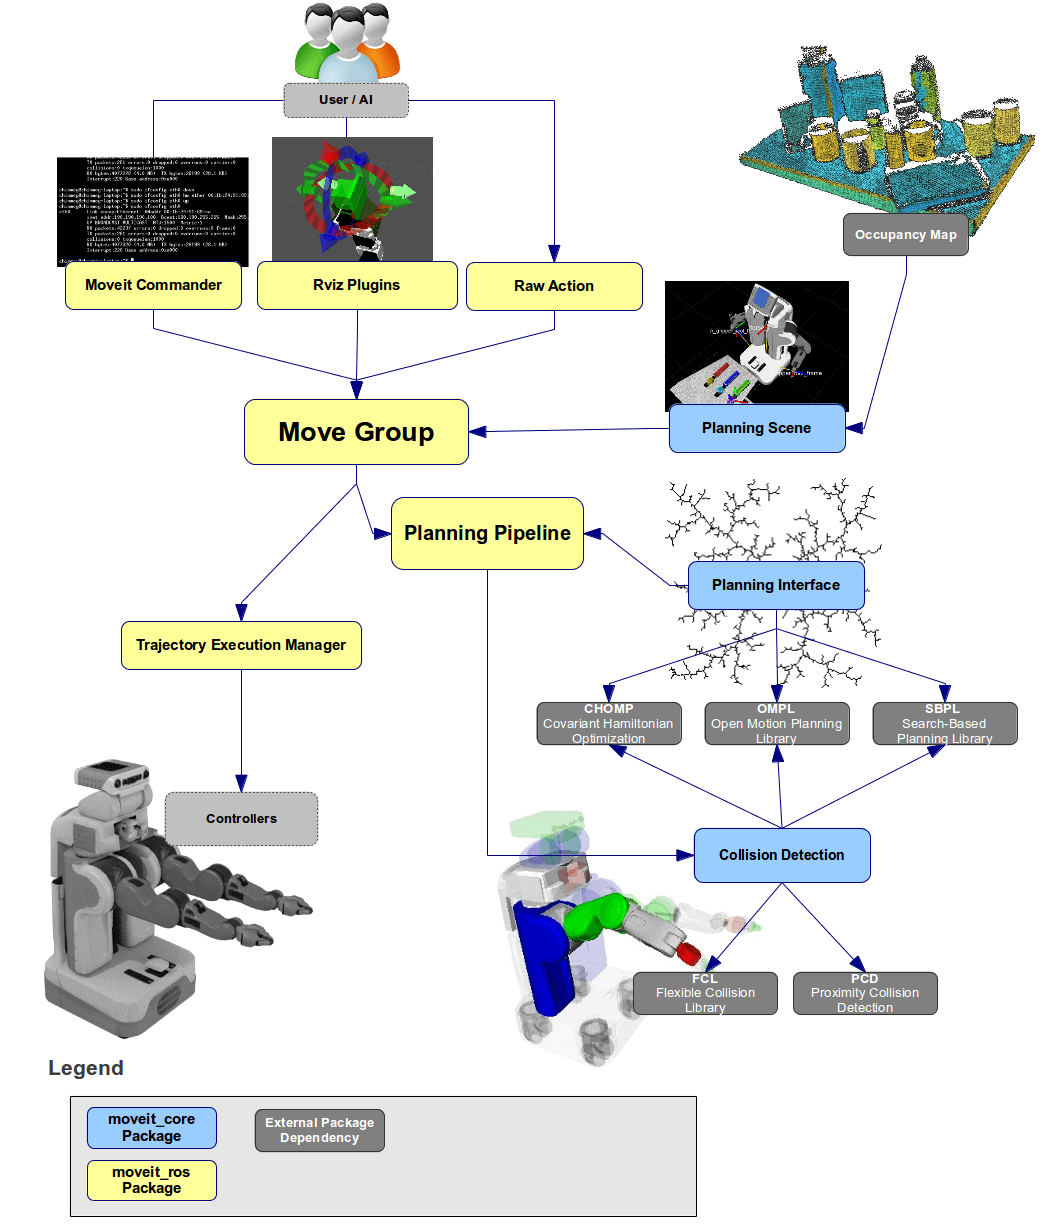
\includegraphics[width=0.8\textwidth]{c4_01.png}
    \caption{MoveIt2 General Architecture}
    \label{fig:moveit2}
\end{figure}

MoveIt2 is a ROS2 framework that provides a set of tools for motion planning, kinematics, control, perception, and
manipulation. It is a powerful tool for controlling robotic arms and mobile bases, and it can be used to plan and
execute trajectories for the arm. MoveIt2 is based on the ROS2 middleware and provides a flexible and modular
framework for developing robotic applications.

The figure \ref{fig:moveit2} shows the general \textbf{architecture of MoveIt2}. The MoveIt2 framework consists of several
components, including the Planning Scene, the Planning Pipeline libraries, the Kinematics Solver, the Collision
Checker, the Trajectory Execution Manager, and the Occupancy Mapping tools.
The Planning Scene is a representation of the robot's environment, including the robot's state, the obstacles in the
environment, and the robot's kinematic model. The diagram in figure \ref{fig:planninscence} shows the architecture
of the Planning Scene and the modules with which it interacts.
The Planning Pipeline libraries are used to generate motion plans
for the robot, using the robot's kinematic model and the obstacles in the environment. The Kinematics Solver is
used to compute the robot's joint positions for a given end-effector pose, using the inverse kinematics
computations based on the robot's kinematic model. The Collision Checker is used to check for collisions between
the robot and the obstacles in the environment, using the robot's kinematic model and the obstacles' geometries.
The Trajectory Execution Manager is used to execute the motion plans generated by the Planning Pipeline libraries,
using the robot's joint positions and velocities. The Occupancy Mapping tools are used to generate volumetric 3D 
occupancy maps of the surrounding environment, using depth perception sensors to construct a map
of the obstacles in the environment. 

\begin{figure}[t]
    \centering
    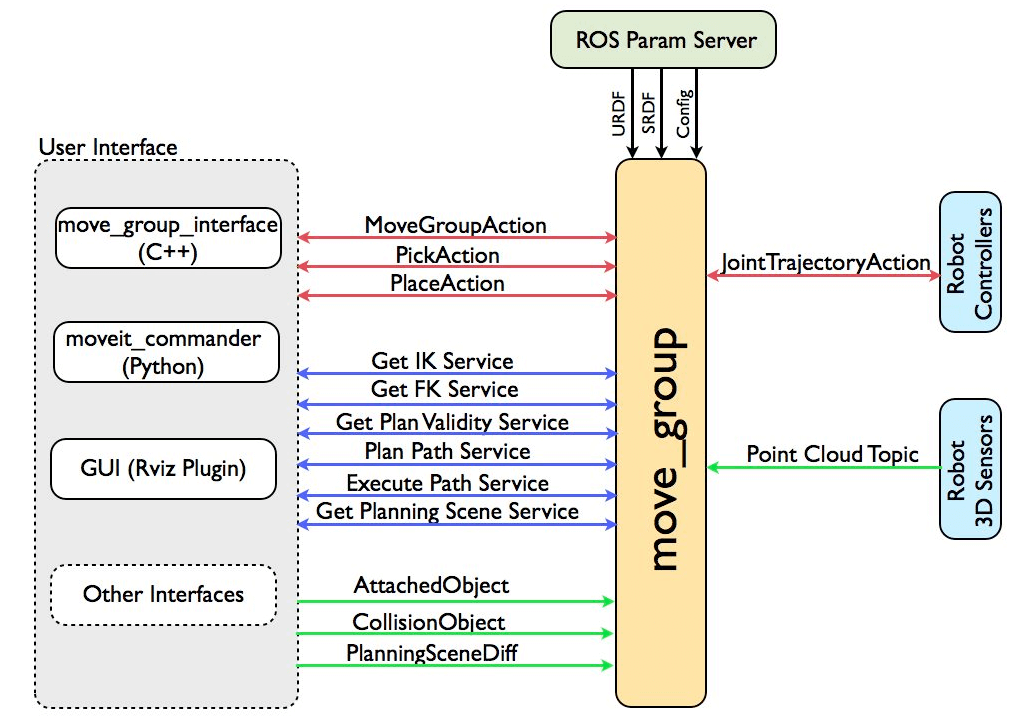
\includegraphics[width=0.8\textwidth]{c4_02.png}
    \caption{MoveGroup Interface}
    \label{fig:move_group}
\end{figure}

MoveIt2 provides the \textit{MoveGroupInterface} class, which is a high-level interface to the MoveGroup node, which is the
class that provides a set of methods for controlling the robot's motion planning and execution. 
Figure \ref{fig:move_group} shows the architecture and the modules with which it interacts.
The \textit{MoveGroupInterface} provides also methods for interacting with the robot's planning scene, 
including adding and removing obstacles, setting the robot's state, and setting the robot's end-effector pose. 
The \textit{MoveGroupInterface} can be used to plan and execute trajectories for the robot. 
It allows to define and compute joint-space goals, Cartesian-space goals,
and pose goals for the robot's end-effector, which is used to compute the joint space trajectories.

%Add a figure of the control architecture
\begin{figure}[t]
    \centering
    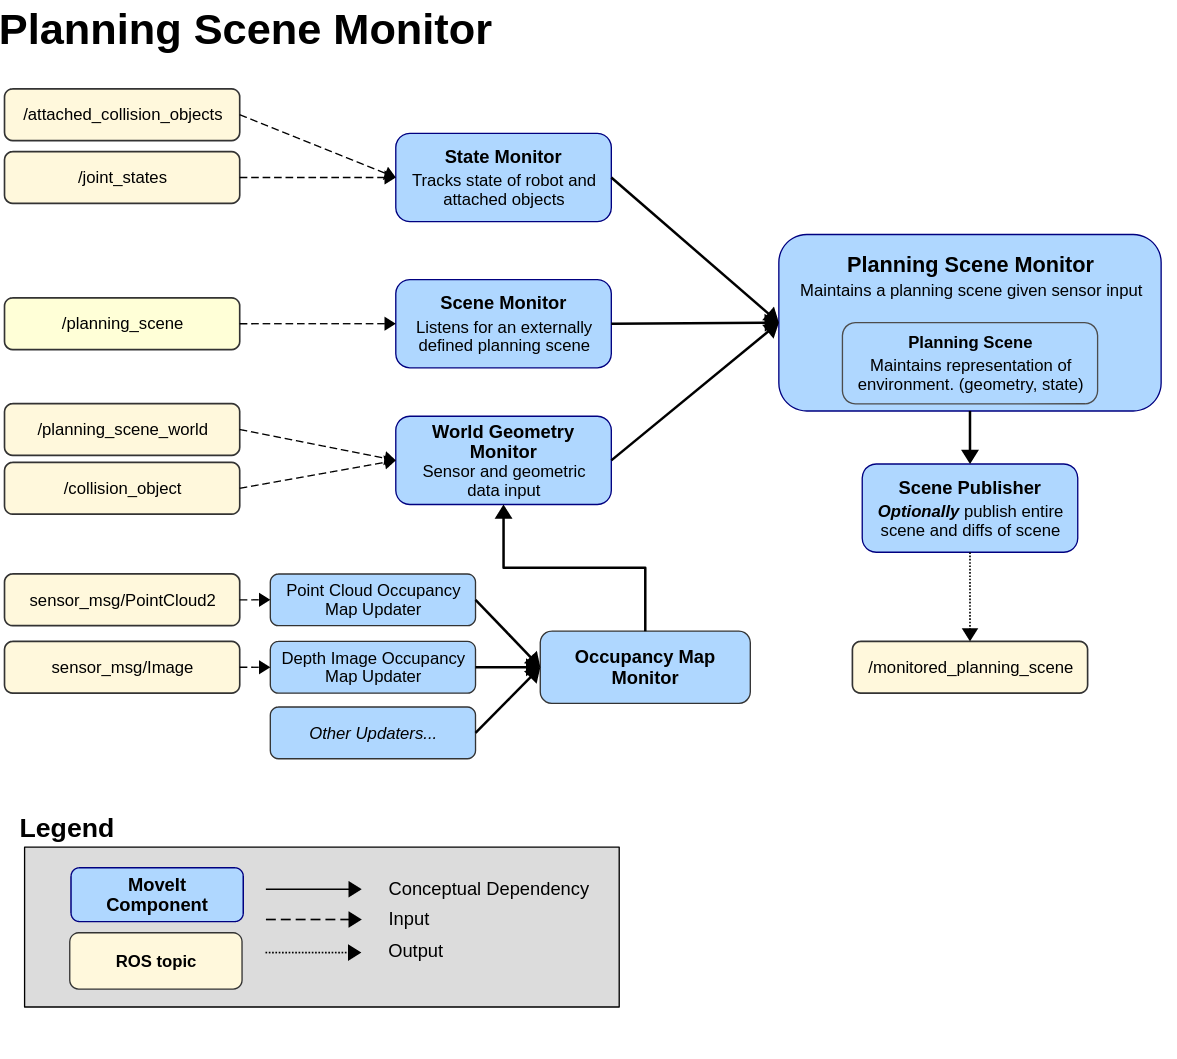
\includegraphics[width=0.8\textwidth]{c4_03.png}
    \caption{Planning Scene and Occupancy Mapping Architecture}
    \label{fig:planninscence}
\end{figure}

MoveIt2 can be used along with RViz2, which is a 3D visualization tool for ROS2 that can be used to visualize the
robot's motion in both simulated and real environments. RViz2 provides a set of tools for visualizing the robot's
kinematic model, the robot's state, the obstacles in the environment, and the robot's motion plans.
Figure \ref{fig:rviz2} shows a screenshot of the RViz2 interface with the control panels dedicated to the MoveIt2
planning and execution tools. With this interface, it is possible to send joint space goals to the robot
and control it via the underlying hardware interface.

%TODO: Add a figure of the rviz2 interface with moveit2
\begin{figure}[t]
    \centering
    %\includegraphics[width=0.8\textwidth]{c4_00.png}
    \caption{RViz2 Interface with MoveIt2 Control Panels and the mobile manipulation robot.}
    \label{fig:rviz2}
\end{figure}

\section{Robotic Arm Visual Servoing}

The MoveIt2 library provides also a framework for visual servo-ing, which is a technique used to control the robot's
end-effector pose using visual feedback from a camera. The visual servo-ing framework in MoveIt2 is based on the
\textit{MoveItServo} package, which provides a set of tools for controlling the robot's end-effector pose using
servo-ing algorithms. The servo-ing algorithms are used to compute the robot's joint positions for a given end-effector
pose. I developed the code to integrate these tools with the camera visual feedback, in order to perform visual servo-ing
experiments with the Igus Rebel Arm. 

The servo-ing algorithms provided by MoveIt2 allow also for \textbf{real-time control and teleoperation} of the robot arm's
end-effector pose. The teleoperation allows the user to control the robot's end-effector pose using a joystick controller.
The real-time control allows the user to control the robot's end-effector pose using camera visual feedback
in real-time without pre-computing the joint trajectories. Realtime control is useful for controlling the robot's
end-effector pose in dynamic environments, where the obstacles are moving and the robot needs to adapt to the changes
in the environment.

\begin{figure}[t]
    \centering
    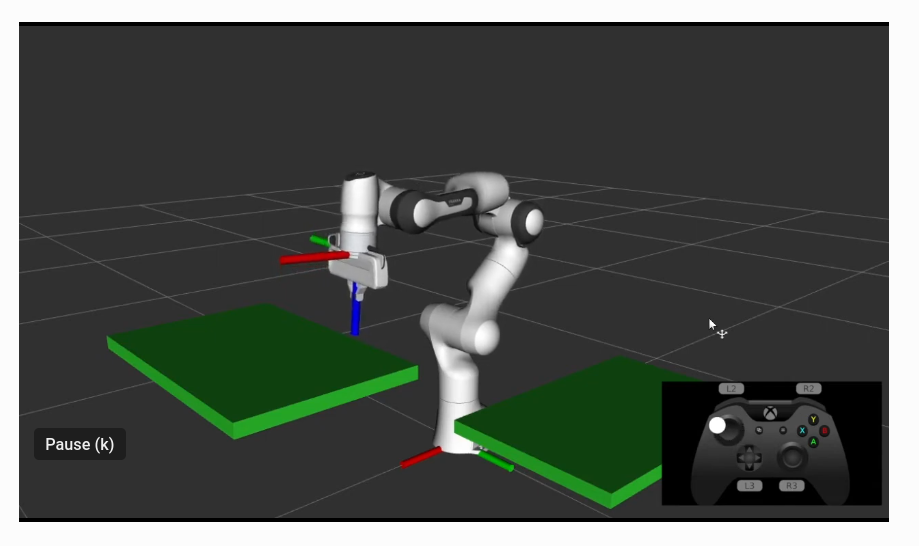
\includegraphics[width=0.8\textwidth]{c4_05.png}
    \caption{Teleoperation with a joystick controller in RViz2 with the Franka Emika Panda}
    \label{fig:teleop}
\end{figure}


After many trials and errors, I managed to get the \textbf{visual servo-ing} working
only with input cartesian poses close to the initial pose of the arm. The servoing algorithm requires
a good initial guess of the end-effector pose, in order to converge to the desired pose.
Since I tested the visual servo-ing with the arm in the open-loop mode, the servo-ing algorithm was not able to
compensate for the errors in the joint positions, which led to the arm not reaching the desired pose.
Then I switched to the closed-loop mode, but the PID controller gains were not tuned properly, which led to strong
oscillations in the joint positions and the arm not reaching the desired pose stably. I did not manage to find the
best gains for the PID controller, so I had to abandon the visual servo-ing experiments with the arm.
The package is still available in the repository, but it is not used in the final implementation
of the mobile manipulation robotic system. Furthermore, the servo-ing algorithms using cartesian input poses
rely exclusively on ROS2-Iron distribution.

\section{Collision Avoidance with Octomap}

The MoveIt2 library provides a framework for collision avoidance using the Octomap library, which is a library for
generating volumetric 3D occupancy maps of the surrounding environment.
Octomap is a 3D probabilistic occupancy grid representation of the robot's environment. It divides the space into voxels
(3D cubes) and assigns probabilities to each voxel, indicating whether it's occupied (by an obstacle) or free.
MoveIt2 integrates data from various sensors, such as the depth camera to update the Octomap in real time.

MoveIt2's collision checker uses the Octomap to efficiently check for collisions between the robot's planned trajectory
and the environment. By checking if the voxels along the path are occupied, it can determine if the robot will collide 
with any obstacles. The probabilistic nature of Octomap helps deal with sensor noise and uncertainty. 
If a voxel has a high probability of being occupied, it's treated as an obstacle.

MoveIt2's motion planners, such as \textit{OMPL} (Open Motion Planning Library), use the Octomap
to generate collision-free paths. The planners avoid occupied voxels to ensure the robot's motion doesn't lead to collisions.
If the environment changes during execution (e.g., an obstacle moves), MoveIt2 can use the updated Octomap 
to quickly replan a new collision-free path, allowing for dynamic obstacle avoidance.
This allows for a dynamic representation of the environment, even if obstacles move.

%TODO: Add a screenshot of the Octomap in RViz2

However, the reality is far from the ideal scenario. The Octomap library is not yet fully integrated with the MoveIt2
interfaces, resulting in a \textbf{poorly optimized} Octomap probabilistic representation of the environment.
In fact, the library takes track of the free space as well as the occupied space, resulting in a memory and computationally
intensive update process, meaning that the time taken for each Octomap update is very high. The Octomap
library for ROS2 is a porting of its ROS1 counterpart, which is fully functional but still lacks some features.
One of the features that are missing is the ability to update the Octomap in realtime when part of the
environment changes. In the current version of the software, Octomap will only update a few voxels around the
part of the environment that changed, without fully removing the voxels corresponding to the obstacle that moved
and that is not present in the scene anymore. This leads to \textbf{false positives in the collision checking}, which
prevents the robot from executing the planned trajectory. This feature is critical for dynamic obstacle avoidance
because the robot needs to avoid the voxels corresponding to the obstacles and touch the voxels corresponding
to the object that the end effector needs to grasp. This means that not only does the robot need to avoid the obstacles
but also understand which voxels the robot arm can collide with.
The Octomap Library is still under development, and it is expected to be correctly integrated with MoveIt2 in the future.

\section{Soft Gripper Pneumatic Pump Actuation}

The soft gripper is actuated using a ROS2-control interface that acts as a hardware interface to the Arduino UNO
microcontroller that controls the pneumatic pump. The hardware interface works by providing a ROS2 service server that 
listens for commands to open or close the gripper and sends the corresponding commands to the Arduino UNO microcontroller
via serial communication. 
The serial communication handles with the UART protocol, which is used to send and receive string messages.
The serial data transfer is done using the \textit{thermios} library, which is a POSIX-compliant library for serial
communication in Linux, supporting the C language.

The Arduino UNO microcontroller is programmed to control the pneumatic pump by changing
the state of the relays connected to its digital pins. The Arduino UNO listens in the serial port for string commands
that it interprets as the pins to be set high or low, to open or close the gripper. The pneumatic pump is connected
to the Arduino UNO via a relay module with 4 relays, one for each digital pin of the pump. Two of which
are the VCC and GND pins, and the other two are the GRIP and RELEASE pins. The GRIP pin is used to close the gripper,
while the RELEASE pin is used to open the gripper.

\section{Autonomous Navigation with NAV2}

Nav2 is a powerful open-source software framework used for autonomous navigation within the ROS2 ecosystem.
It provides a comprehensive set of tools and algorithms for enabling robots to navigate complex environments intelligently.
With Nav2, robots can perceive their surroundings, localize themselves, plan optimal paths, and execute 
those paths while avoiding obstacles. Its modular architecture allows for customization and integration with various sensors,
such as LiDAR and cameras, making it adaptable to different robot platforms and use cases. 
Nav2's flexibility and robust features make it a popular choice for both research and industrial applications 
in fields like robotics and autonomous vehicles.

Nav2's \textbf{modular architecture} enables the seamless integration of various plugins that contribute
to its robust autonomous navigation capabilities. Costmap plugins, such as static and obstacle layers,
create a real-time representation of the robot's environment, highlighting obstacles and free space. 
Collision monitors continuously assess the robot's planned path against this costmap ensuring safe navigation.
Localizers, like AMCL, estimate the robot's position within the environment, while mappers like SLAM create and update maps
of the surroundings. Planners, such as global planners (e.g., Hybrid A*) and local planners (e.g., DWB),
work in tandem to generate collision-free paths for the robot to follow, enabling efficient and fast navigation. 
Additionally, plugins like controllers and recovery behaviors further enhance Nav2's ability to handle unexpected
scenarios and ensure the robot reaches its goal.

Given these premises and features, I decided to use Nav2 as the primary navigation stack for the mobile manipulation
robotic system. The Nav2 stack is used to plan and execute trajectories for the mobile base, using the robot's
LiDAR sensor to perceive the environment and avoid obstacles. The stack operates within a ROS2 
composable node architecture, which allows for the integration of various plugins and algorithms to achieve
efficient intra-process communication and data sharing between the various components and threads of the stack.

%TODO: add screenshot of map and costmaps in RViz2

\subsection{Nav2 Parameters Tuning}

Finding the right parameters for the Nav2 stack was a challenging task, as the stack has many parameters that need
to be tuned to achieve optimal performance. The parameters to be set are related to all the plugins that are part
of the Nav2 stack. Many tests in different and complex environments were performed to find the best parameters
suitable for the AgileX Scout robot. The parameters were set based on many days of intense testing in both simulated
and real environments, to ensure that the robot can navigate safely and efficiently in different scenarios.

\textbf{Localization Algorithms}:
I tested and applied both AMCL and SLAM Toolbox algorithms for localization, and I found that the AMCL algorithm
performed worse in terms of scan matching when the robot rotates in place. Therefore, I decided to use the SLAM Toolbox
algorithm for localization, which provided better performance and improved reliability in terms of localization accuracy,
even in maps with dynamic obstacles and changing environments.

\textbf{Global Planner}:
I tested and used the Hybrid A* global planner, and I found that it performed well in generating optimal paths
for the robot to follow, even in cases where an unknown obstacle appears in the environment. The Hybrid A*
global planner uses an A* search algorithm to generate optimal paths for the robot to follow, which allows the robot
to compute efficient paths and adjust quickly to changes in the environment. The Hybrid A* global planner is based on
the motion generation algorithm, which generates kinematically feasible paths for the robot to follow, and the path selection
algorithm, which selects the best path from the sample paths based on the cost function.
The motion generation algorithms available are the \textit{Dubin} and \textit{Reeds-Shepp} algorithms, which both generate
kinematically feasible motion trajectories. After many tests, I found that the Reeds-Shepp algorithm enabled
to generate paths also in the reverse direction, which is useful for navigating in reverse, especially for
a skid-steering drive robot such as the Scout. However, for some reason still unknown to mankind and Steve Macenski,
the Reeds-Shepp algorithm works only in the real environment, and not in the simulated environment in Ignition Gazebo.

\textbf{Local Planner (Controller)}:
I tested and applied the DWB and MPPI local planners, and I found that the MPPI local planner performed better
in tracking the global plan and avoiding tight obstacles. The MPPI (Model Predictive Path Integral Controller) 
local planner uses a \textbf{model predictive control approach}
to generate collision-free paths for the robot to follow, which allows the robot to navigate efficiently in complex
environments with tight spaces and obstacles. The MPPI local planner also provides better performance in terms of
trajectory tracking, compared to the DWB local planner. The DWB local planner uses a dynamic window approach to generate
collision-free paths for the robot to follow, which can be less effective in tight spaces and complex environments.

\textbf{Recovery Behaviors}:
I tested the default recovery behaviors provided by the Nav2 stack, and I found that the default recovery behaviors
performed well in recovering the robot from unexpected scenarios, such as getting stuck or colliding with obstacles.
So I decided to modify slightly the default recovery behaviors to improve the robot's performance in recovering
from the scenarios where the robot would be stuck near an obstacle and unable to move. The modified recovery behaviors
include a combination of back-up and rotate behaviors, which allow the robot to back up and rotate in place to position
itself in a different configuration, enabling it to generate a new path and continue navigating towards the goal.

\textbf{Local Costmap}:
The local costmap plugin is used to generate a local costmap of the robot's surroundings, highlighting obstacles
and free space. The local costmap plugin uses the robot's LiDAR sensor to perceive the environment and update the costmap
in realtime. The local costmap plugin is used by the local planner to generate collision-free paths for the robot
to follow. The local costmap can be configured with these plugins:

\begin{itemize}
    \item \textbf{Inflation Layer}: The inflation layer is used to inflate the obstacles in the costmap, creating a buffer
    around the obstacles to ensure that the robot avoids collisions.
    \item \textbf{Obstacle Layer}: The obstacle layer is used to update the costmap with the obstacles detected by
    the 2D LiDAR sensor, highlighting the obstacles in the costmap. I later substituted this layer with the voxel layer,
    thanks to the more effective 3D LiDAR sensor perception.
    \item \textbf{Static Layer}: The static layer is used to update the costmap with the static obstacles in the map
    \item \textbf{Voxel Layer}: The voxel layer is used to update the costmap with the voxelized obstacles in the map,
    using the 3D LiDAR sensor to perceive the environment and update the costmap in realtime.
\end{itemize}

\textbf{Global Costmap}:
The global costmap plugin is used to generate a costmap of the entire map that the robot is navigating in, highlighting
the static obstacles and free space. The global costmap plugin is used by the global planner to generate optimal paths
for the robot to follow. The global costmap is configured to use only the static layer inflated by the inflation layer,
to ensure that the robot avoids collisions with the obstacles already present in the map.

\textbf{Collision Monitor}:
The collision monitor plugin is used to continuously assess the robot's planned path against the costmap, ensuring
that the robot navigates safely and avoids collisions with obstacles. The collision monitor plugin is used by the
nav2 stack to ensure that the robot avoids the obstacles in the costmap, such that they do not overlap with the robot's
footprint and locally planned path.

\textbf{Mapping Algorithm}:
The algorithm of choice for mapping is the \textit{SLAM Toolbox} algorithm, which is a 2D SLAM algorithm
that uses the robot's LiDAR sensor to create a 2D map of the environment. The SLAM Toolbox algorithm is used to create
a 2D map of the environment, which is used by the global planner to generate optimal paths for the robot to follow.
The SLAM Toolbox proved to be effective in creating accurate 2D maps of the environment, even in dynamic environments
with moving obstacles. I managed to use it correctly in both simulated and real environments, and it provided
good performance in terms of mapping accuracy and reliability.

\textbf{Velocity Smoother}:
The velocity smoother plugin is used to smooth the robot's velocity commands, ensuring that the robot moves smoothly
and efficiently in the environment. The velocity smoother plugin is used by the local planner to obtain smooth
trajectories from the computed paths, which allows the robot to navigate efficiently and avoid jerky movements.
The velocity smoother is configured also to avoid unnecessary stops and starts, which can wear out the robot's transmission
gears and reduce the robot's battery life.

\textbf{Spatio-Temporal Voxel Costmap Layer}:
The dynamic obstacle avoidance algorithm is a critical component of the Nav2 stack, as it allows the robot to navigate
safely in dynamic environments with moving obstacles. The dynamic obstacle avoidance algorithm uses the robot's LiDAR sensor
to perceive the environment and detect the moving obstacles in realtime. Dynamic obstacles update the local costmap
following different plugins, such as the voxel layer, which is used to update the costmap with the voxelized obstacles
in the environment. The voxel layer uses the 3D LiDAR sensor to perceive the environment and update the costmap.
However, one of the shortcomings of the voxel layer is that it doesn't remove old voxels that correspond to obstacles
that are no longer present in the environment. This leads to false positives in the collision checking, which prevents
the robot from executing the planned trajectory, especially in highly dynamic environments with fast-moving obstacles.
The spatio-temporal voxel costmap layer is an open-source plugin that addresses this issue by updating the costmap
efficiently and accurately. It replaces the traditional voxel grid approach with a \textbf{sparse voxel grid} implemented
using OpenVDB, a high-performance C++ library. This allows STVL to handle large, dynamic environments with ease,
such as the one shown in figure \ref{fig:stvl}, 
reducing computational overhead. By leveraging temporal information and applying a voxel grid filter to sensor data,
STVL can better handle noisy and dense sensor readings, especially in proximity to objects. 
This results in smoother, more reliable navigation and improved robot performance in continuously evolving scenarios.
STVL's adaptability, efficiency, and ability to integrate with various sensor types made it the ideal substitute
for the voxel layer in the Nav2 stack.

\begin{figure}[t]
    \centering
    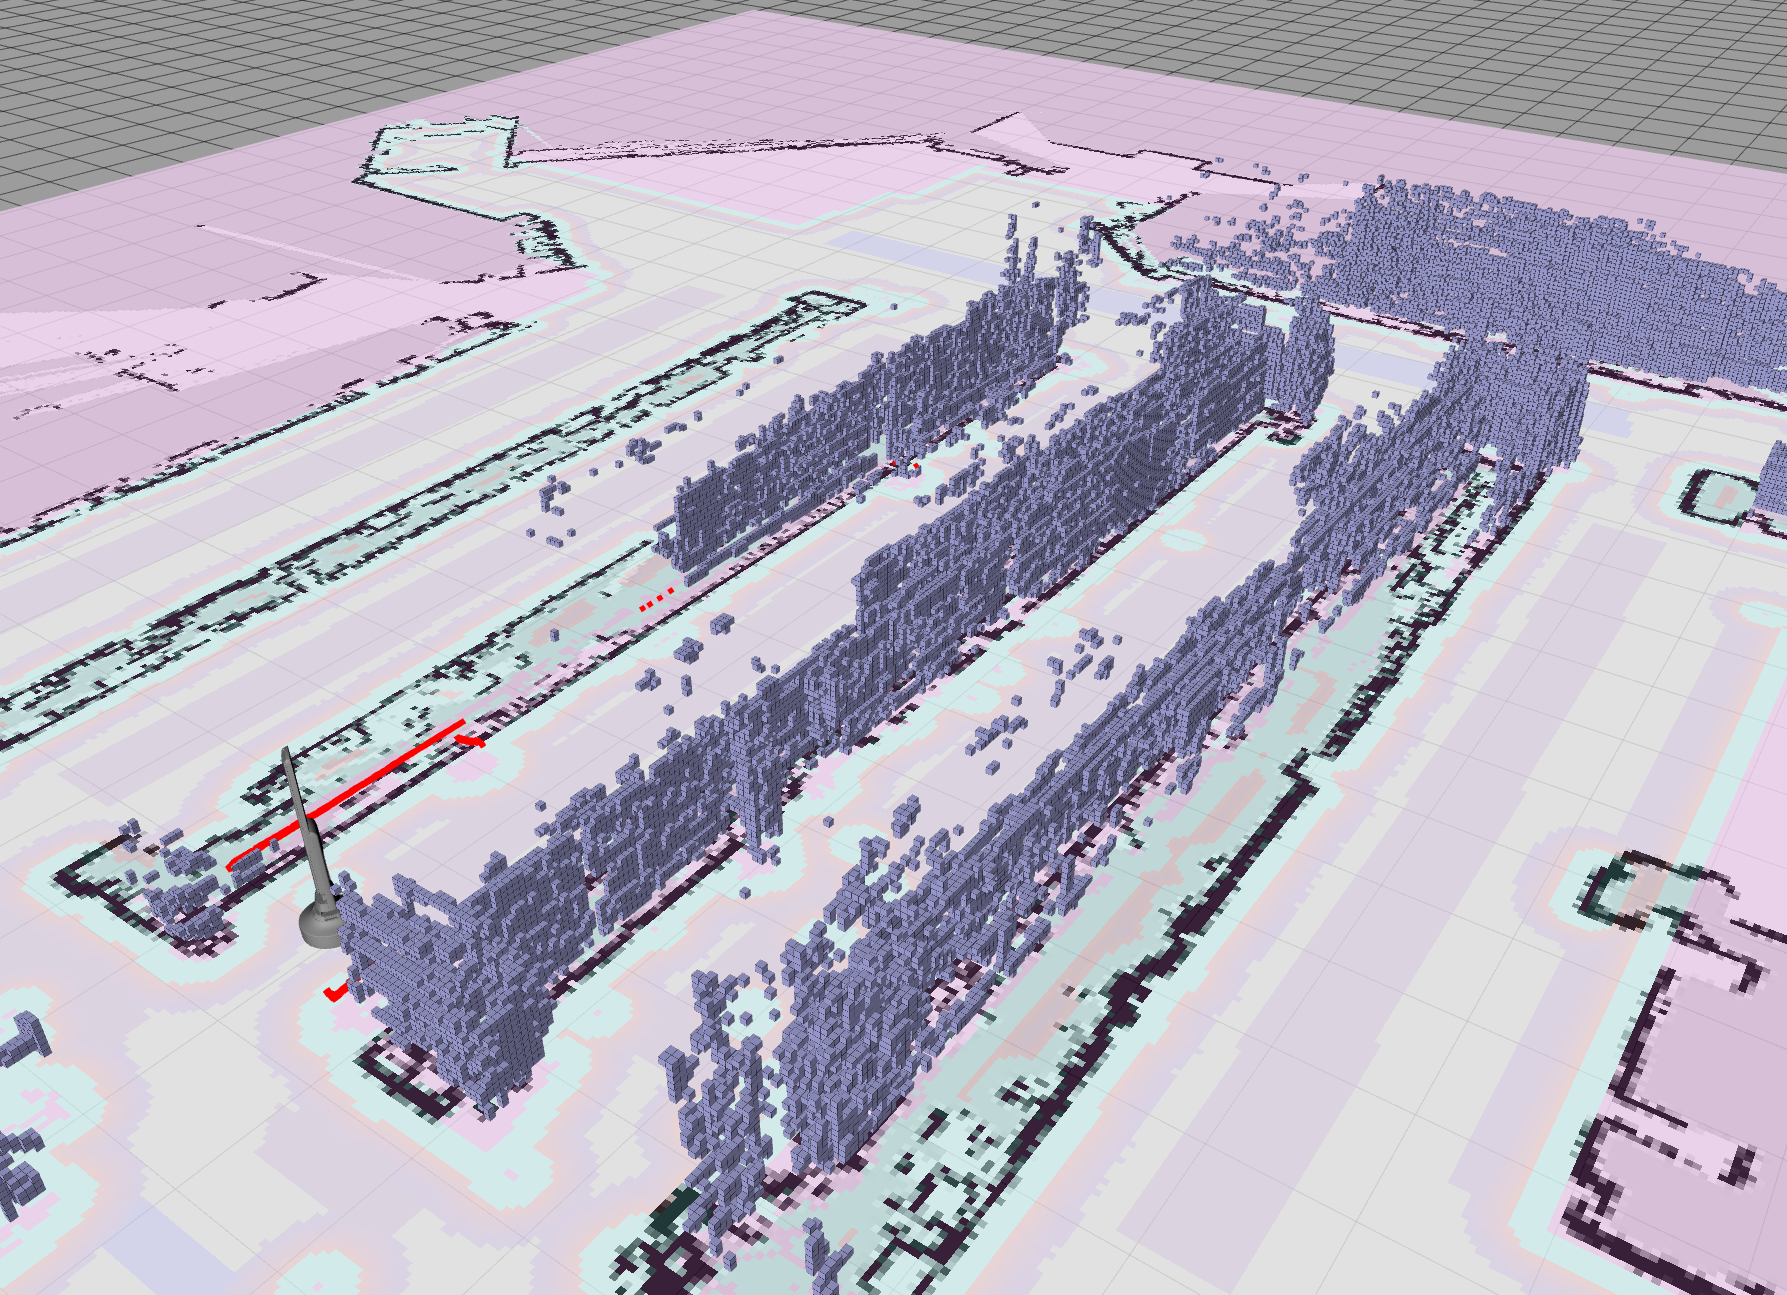
\includegraphics[width=0.8\textwidth]{c4_06.png}
    \caption{STVL in action in a dynamic and cluttered warehouse environment}
    \label{fig:stvl}
\end{figure}


\subsection{Issues with 3D LiDAR for autonomous navigation}

Throughout the development of the project, I encountered several issues with the NAV2 stack.
Sometimes the software crashed at random times, unpredictably, and without any apparent reason.
Some other times the dynamic obstacle avoidance algorithm did not work as expected, causing the robot to collide
with obstacles that were not perceived by the LiDAR sensor in the surrounding environment.
Overall, the robot's navigation stack was not reliable and robust, which was a significant issue for the project's development,
especially for the autonomous navigation tasks in the laboratory's environment (cluttered and dynamic).

After many trials and tests, my supervisor and I discovered that the LiDAR pointcloud data's low and unreliable frequency
was the main cause of all these problems. The LiDAR sensor works at a nominal frequency of $10$Hz. 
The LiDAR sensor was not providing a stable scan rate of $10$Hz, but it was fluctuating between $3$Hz and $8$Hz, 
and only in a few cases, it was able to provide the nominal $10$Hz scan rate.
Once we discovered the source of the problem and ensured that the LiDAR sensor was working correctly
(meaning that the sensor was not malfunctioning or working at a lower but valid data rate), 
we tried to find the culprit of the low and unreliable frequency of the LiDAR sensor.

After many attempts, I found out the cause of the problem: the culprit was the \textbf{router}
used to connect the robot's computer
to the laboratory's network and the internet and the DDS (\textit{Data Distribution Service}) middleware used 
internally by ROS2 for the communication between the nodes in a local network. Basically, the DDS middleware
was configured to broadcast all ROS2 packets and data streams to the laboratory's network, causing delays in the transmission
and packet loss, as the network was not able to handle the high-frequency and heavy-weight data streams of the LiDAR sensor.
In fact, by just unplugging the router from the robot's computer, the LiDAR sensor was able to provide a stable scan rate
of $10$Hz, without any fluctuations or drops in the frequency, since no broadcast packets were sent to the network.
Since the router was necessary for the remote control and monitoring, it was simply just not an option
to unplug it from the robot's computer.

For the correct operation of the localization and obstacle 
avoidance algorithms, it is fundamental that the LiDAR sensor works at a \textbf{stable frequency}, 
without any fluctuations or drops in the scan rate. This requirement is essential because these algorithms rely on the
coherent and continuous data stream for time interpolation and filtering of the pointcloud data.
This is why the LiDAR sensor's low and unreliable frequency was causing the software to crash and malfunction.

The solution was to configure properly the \textbf{DDS middleware} to ensure that all ROS-related nodes and data streams
were handled inside the robot's computer only, and not going through the router and the laboratory's network.
Having the data streams in the local machine only, ensured that the LiDAR sensor's data was not distributed 
among the network, causing delays in the transmission and packet loss, which were the main causes of the low and unreliable
frequency of the LiDAR sensor. Furthermore, we configured ROS2 to use the \textit{Cyclone DDS} middleware, which is a lightweight
and fast DDS implementation, suitable for real-time and high-frequency data streams. This DDS implementation was able to handle
heavy-weight data packets at high frequencies, ensuring that the LiDAR sensor's data was transmitted and received correctly
in its entirety, without any losses or delays in the transmission.

After this configuration, the LiDAR sensor was able to provide a stable scan rate of $10$Hz,
and the software stack was working correctly, without any crashes or malfunctions.
Furthermore, I was also able to test the LiDAR sensor at a higher frequency of $20$Hz, 
with lower resolution, and it was working fine and stable.
This solution was essential also for the correct operation of the IMU sensor for the SLAM algorithm, which required
a stable and continuous data stream of the LiDAR at the moment of startup of the sensor in the software stack. Before the 
fix of the LiDAR sensor's frequency, the IMU sensor was not able to start correctly, due to the lack of data
from the LiDAR sensor, and the computed odometry data was drifting too much to be useful.
Many other algorithms and software benefitted from this fix. The robot's navigation stack was now reliable and robust,
and the autonomous navigation tasks were working correctly and smoothly.


\section{Ignition Gazebo Simulation Environment}

Ignition Gazebo is a useful open-source simulation environment for robotics and autonomous systems.
It provides a realistic and customizable 3D environment for testing and developing robotic algorithms and applications.
Ignition Gazebo is the new version of the Gazebo simulator, which is widely used in the robotics community for simulating
robots and sensors for perception systems. Ignition Gazebo was the simulation environment of choice for the project,
as it proved to be very useful in testing the mobile robot base in simulated environments before deploying the algorithms
on the real robot. Simulating the robot in a virtual environment allows for testing the algorithms in 
a controlled and repeatable environment, without the risk of damaging the real robot or the laboratory environment.
It was essential for the development of the software stack and the navigation algorithms, as it allowed for testing
the robot's behavior in different scenarios and environments. It allowed me to tune the navigation stack's parameters
thoroughly and ensure the robot would avoid obstacles and navigate safely.

The simulated environment in Ignition Gazebo was a warehouse with various obstacles such as walls, shelves, and boxes,
which the robot had to navigate around to reach its goal. The warehouse environment was designed to be challenging
for the robot, with narrow passages and tight spaces, to test the robot's ability to navigate in complex environments.
Ignition Gazebo also provides the possibility to add dynamic obstacles, i.e. objects not present in the map
already loaded in the simulation environment. This feature was useful for testing the robot's dynamic obstacle avoidance
algorithm, which allows the robot to navigate safely in environments with unknown obstacles.

I was able to simulate also the sensors mounted on the robot, such as a 2D LiDAR and a 3D LiDAR sensor, which were used
for perception and obstacle avoidance. I also tested the robot's localization algorithms, such as AMCL and SLAM Toolbox,
using the simulated odometry data created by the robot's motion in the simulated environment.

%TODO: add a screenshot of the simulation environment in Ignition Gazebo

%TODO: add the created map of the warehouse

\section{Parking Algorithm for Mobile Robot}

I designed a parking algorithm for the mobile robot to autonomously park near a target spot in the laboratory.
The parking algorithm takes as input the location in the map of the target spot that the robotic arm must reach,
and it outputs the parking pose next to the target pose where the mobile robot must park to give the robotic arm
enough space to reach the target. I had to structure and design the algorithm to ensure that the mobile robot
could park in a position where the robotic arm could interact with the target object, without colliding with 
the obstacles in the environment nor with the target object itself. The mobile robot must park so that it 
faces the opposite direction of the target object because the robotic arm is mounted on the back of the robot.

The parking algorithm considers both the robot's footprint and the robotic arm's workspace to ensure that the
robot can park in a position where the robotic arm can reach the target object. 
The algorithm also considers the costmap generated by the navigation stack to compute the optimal parking
pose that minimizes the cost of the footprint, meaning that the robot will be the furthest possible from
the obstacles in its vicinity. 

The parking algorithm is then used by the NAV2 commander APIs to send the parking pose to the robot's navigation stack,
which generates a collision-free path for the robot to follow to reach the parking pose. The robot then executes
the planned trajectory and parks near the computed parking pose. While the mobile robot navigates
autonomously to the parking pose, it publishes feedback data containing its current position and its distance 
from the parking pose. 

The parking algorithm is non-deterministic, meaning that it can compute different parking poses for the same target
pose, depending on the obstacles in the environment. It works as follows:

%TODO: add pseudo code of the parking algorithm

Experimental tests were performed to evaluate the accuracy and reliability of the parking algorithm.
The tests were conducted in both simulated and real environments, with different configurations of obstacles
and target poses. The parking algorithm was able to compute effective parking poses in most cases,
but it struggled with tight spaces and narrow passages, where the robot had limited space to park.
The biggest limitation of this algorithm is that it cannot consider the feasible workspace of the robotic arm
when computing the parking pose, which can lead to the robot parking in a position where the robotic arm
cannot reach the target object. This limitation is due to the impossibility of predicting the cartesian
target pose that the cobot will have to reach, as it depends on the object's position and orientation
in the environment. The parking algorithm is a good starting point for further development and improvement
to address these limitations and ensure that the robot can park in a useful position also for the robotic arm.

\section{Aruco Marker Detection and Pose Estimation}

Aruco markers are synthetic square markers with unique black-and-white patterns that can be easily detected
and identified by computer vision algorithms.

Detecting and estimating the pose of an ArUco marker from an image involves a two-step process.
First, the ArUco marker is detected in the image using the ArUco library available in OpenCV. 
This library provides functions to detect various ArUco dictionaries and families. 
Once detected, the marker's corners are extracted, and its unique ID is identified. 
The second step involves estimating the pose of the ArUco marker, which refers to its position 
(translation) and orientation (rotation) with respect to the camera. The function for pose estimation 
takes the detected marker corners, the marker size, and the camera's intrinsic parameters (focal length,
principal point, and distortion coefficients) as input and returns the pose of the marker in the form of a rotation
vector and a translation vector.

The intrinsic parameters of the camera are crucial for accurate pose estimation. These parameters describe the camera's
internal characteristics, such as the focal length, which determines the field of view, and the principal point,
which is the center of the image. The distortion coefficients model the lens distortion, which can cause straight
lines to appear curved in the image. By incorporating these parameters into the pose estimation process,
we can compensate for the camera's inherent distortions and obtain a more accurate estimate of the ArUco marker's pose
in the real world. I had also to calibrate the camera's intrinsic parameters using a calibration pattern and the
automatic calibration software tool provided by the RealSense SDK.

%TODO: add pictures of detected markers

\subsection{Multi-Aruco Plane Estimation Algorithm}

One of the challenges I faced was estimating the orientation of small Aruco markers from the camera feed.
The pose estimation algorithm works well for markers that appear large in the image, but it struggles with
the ones that appear smaller due to the size and distance from the camera. The estimation of the orientation
was the most challenging part, as the pose estimation algorithm often returns orientation values that
oscillate between different values, making it difficult to determine the correct orientation of the marker.
This is especially true for small markers that appear far away from the camera. To address this issue,
I developed a multi-Aruco plane estimation algorithm that estimates the orientation of a plane over which
multiple Aruco markers are placed.

The algorithm works by detecting multiple Aruco markers in the image and estimating their poses using the pose
estimation algorithm. The poses of the Aruco markers are then used to estimate the orientation of the plane
on which the markers are placed. The algorithm assumes that the Aruco markers are coplanar, meaning that 
they have different positions but the same orientation. By estimating the orientation of the plane that passes
through the markers, we can determine the correct orientation of the markers from the vector normal
to the plane. The algorithm processes a list of Aruco markers poses and returns the poses with their
estimated orientation, meaning that all processed poses share the same orientation value.

The algorithm that I implemented makes use of the following statistical data analysis techniques:

\begin{itemize}
    \item \textbf{RANSAC (Random Sample Consensus)}: RANSAC is an iterative algorithm used to estimate
    the parameters of a mathematical model from a set of observed data points that contain outliers.
    RANSAC works by randomly selecting a subset of data points and fitting a model to them. The model is then
    evaluated against the remaining data points, and the points that are consistent with the model are considered
    inliers. The process is repeated multiple times to find the best-fitting model with the maximum number of inliers.
    RANSAC is used to discard the outlier data points observed in the Aruco markers' poses.
    \item \textbf{Least Squares Estimation (LSE)}: LSE is a mathematical method used to find the best-fitting curve
    that minimizes the sum of the squared differences between the observed data points and the model's predictions.
    LSE is used by the RANSAC model to fit the plane that passes through the Aruco markers' poses.
    \item \textbf{Principal Component Analysis (PCA)}: PCA is a statistical method that identifies patterns
    in data by transforming it into a new coordinate system, where the data points are uncorrelated.
    PCA is used to find the principal components of the data, which are the directions of maximum variance.
    In the context of this algorithm, PCA is used to find the vector passing through points lying on a line.
    It is used as a technique for outlier removal and noise reduction in the data.
    \item \textbf{Singular Value Decomposition (SVD)}: SVD is a matrix factorization technique that decomposes
    a matrix into three matrices, which represent the singular vectors and singular values of the original matrix.
    SVD is used as an optimization technique to find the best-fitting plane that passes through the given points.
    It works as a technique for reducing the dimensionality of the data, by reducing the impact of noisy
    and irrelevant data points.
\end{itemize}

The algorithm works as follows:
%TODO: write algorithm description
\begin{algorithm}[H]
    \caption{Multi-Aruco Plane Estimation Algorithm}
    \label{alg:multi_aruco}
    \begin{algorithmic}[1]
    
    \REQUIRE Reference voltage vector $V_{ref}$, sector angle $\theta_{ref}$, modulation index $m$
    \ENSURE Duty cycles $d_a$, $d_b$, $d_c$
    
    \STATE Calculate $x$, $y$, $z$ components of $V_{ref}$:
    \STATE $x \gets m \cdot \cos(\theta_{ref})$
    \STATE $y \gets m \cdot \sin(\theta_{ref})$
    \STATE $z \gets 0$
    
    \STATE Determine the sector ($s$) and the angles ($\theta_1$, $\theta_2$) for the two nearest space vectors:
    \STATE $s \gets \lfloor \frac{\theta_{ref}}{\pi/3} \rfloor + 1$
    \STATE $\theta_1 \gets \theta_{ref} - (s-1) \cdot \frac{\pi}{3}$
    \STATE $\theta_2 \gets \frac{\pi}{3} - \theta_1$
    
    \STATE Calculate the duty cycles for the three phases:
    \STATE $d_a \gets \frac{\sqrt{3}}{2} \cdot m \cdot \sin(\theta_2)$
    \STATE $d_b \gets \frac{\sqrt{3}}{2} \cdot m \cdot \sin(\theta_1)$
    \STATE $d_c \gets 1 - d_a - d_b$
    
    \STATE Normalize duty cycles if necessary:
    \IF{$d_a + d_b + d_c \neq 1$} 
        \STATE $d_a \gets d_a / (d_a + d_b + d_c)$
        \STATE $d_b \gets d_b / (d_a + d_b + d_c)$
        \STATE $d_c \gets d_c / (d_a + d_b + d_c)$
    \ENDIF
    
    \end{algorithmic}
\end{algorithm}

\section{Object Detection with YOLOv8}

For the project, it was also necessary to detect objects in the environment, such as colored balls, which the robot
had to grasp and move to a different location. For this task, I used the YOLOv8 object detection algorithm, trained
on a custom dataset that I collected and annotated.

\textbf{YOLO (You Only Look Once)} is a cutting-edge, real-time object detection algorithm 
that has revolutionized computer vision.
Unlike traditional methods that require multiple passes over an image, YOLO analyzes the entire image in a single pass,
making it incredibly fast and efficient. It divides the image into a grid and predicts bounding boxes and class probabilities
for each grid cell simultaneously, achieving impressive accuracy while maintaining speed. 
YOLO has evolved through several versions (YOLOv2, YOLOv3, etc.), each improving upon the previous iteration in terms of speed, 
accuracy, and ability to detect small objects. Its versatility and effectiveness have led to widespread adoption in various
applications, including autonomous driving, robotics and image analysis tools. This was the object detection neural
network of choice for the project, as it provided the speed and accuracy needed for detecting objects in real-time
from the camera feed. It is also lightweight, making it ideal to run on CPUs without the need for a GPU.
The inference time for a single image on an Intel i7 12th gen CPU was around $0.15$ seconds, which is fast enough
for the time requirements of my applications. However, when running along other ROS2 nodes using other CPU-intensive
algorithms, the inference time increased to $0.4$ seconds, which was still acceptable for the demos and tests.

The YOLOv8 algorithm is a state-of-the-art object detection model that combines the best features of previous YOLO versions
to achieve superior performance. I used this model for my object detection task, such as detecting colored balls
from the camera feed. I trained the YOLOv8 model on a custom dataset of colored balls, which included images of the balls
from different angles, distances, and lighting conditions. I collected the dataset using the RealSense camera mounted
on a tripod, which allowed me to capture images of the balls from different perspectives and distances. The dataset
was annotated manually with the bounding boxes and class labels of the balls, which were used to train the YOLOv8 model.

I used the YOLOv8 model provided by \textbf{Keras}, which is a high-level deep-learning library that provides a user-friendly
API for building and training neural networks. Since the training dataset I collected is of small size,
I used data augmentation techniques to increase the dataset's size and diversity, which helped improve the model's
generalization and robustness. The data augmentation techniques included random rotations, translations, and flips
of the images, which created variations of the original images and helped the model learn to detect the balls
from different perspectives and orientations. I included also other types of image augmentation techniques, such as
brightness and contrast adjustments, and Gaussian noise addition, which further increased the dataset's
size and variability. The image augmentation algorithms were implemented using the \textit{Albumentations} library,
which is a powerful image augmentation library for computer vision tasks, specially designed for 
object detection tasks. It is essential to adjust properly the bounding boxes after each image
is augmented, to ensure that the bounding boxes are still correctly positioned around the objects of interest.

As training hyperparameters, I used a batch size of $16$, which is enough for a small dataset such as the one
that I created, a learning rate scheduler with exponential decay, and the early stopping callback to stop the training
when the validation loss stops decreasing. The model is compiled with the Adam optimizer, which is a popular optimizer
for training deep neural networks, and with the YOLOv8 Backbone, which is a state-of-the-art backbone architecture
that provides the best candidate features for object detection tasks. The metrics used to evaluate the model's performance
are the \textbf{mean Average Precision} (mAP) and the Intersection over Union (IoU),
which are standard metrics for object detection tasks. These metrics are incorporated within the COCO evaluation metrics,
which are the standard evaluation metrics provided by the KerasCV library.

The model is trained with the combination of 2 loss functions:

\begin{itemize}
    \item \textbf{Box Loss}: The box loss function is used to penalize the model for incorrect predictions of the bounding
    boxes of the objects. The box loss function computes the difference between the predicted bounding boxes and the
    ground-truth bounding boxes, using the \textit{CIoU} (Complete Intersection over Union) loss function, which is a
    state-of-the-art loss function that accounts for the object's aspect ratio and orientation.
    \item \textbf{Class Loss}: The class loss function is used to penalize the model for incorrect predictions of the
    object classes. The class loss function computes the difference between the predicted class probabilities and the
    ground-truth class labels, using the \textit{Binary Cross-Entropy} loss function, which is the loss function of
    choice for multi-class classification tasks that use multi-hot encoded labels instead of one-hot encoded labels.
    After some tests, I switched to the \textit{Binary Penalty Reduced Focal CrossEntropy} loss function, which is a variant
    of the focal loss function that reduces the penalty for misclassifications, and focuses more on the correct
    classification of the objects. This loss function helped improve the model's accuracy.
\end{itemize}


%TODO: add pictures of detected balls

\section{Object Pose Estimation with Object Detection and Depth Sensing}

\section{ROS2 Actions Client-Server Architecture for High-Level Tasks}

